 La medición del consumo energético de un sistema consiste en la recopilación de métricas relacionadas con su funcionamiento para, posteriormente, procesar los datos obtenidos y determinar diferentes magnitudes, entre las que destacan la \textbf{potencia} y la \textbf{energía consumida}. La \textit{potencia} representa la cantidad de energía que un sistema consume o transforma por unidad de tiempo y se expresa habitualmente en vatios (W). Por su parte, la \textit{energía consumida} representa la cantidad total de energía utilizada por el sistema durante un periodo de tiempo determinado o para llevar a cabo una tarea concreta. Esta magnitud se expresa principalmente en julios (J) o en vatios-hora (Wh).
 
 A partir de estas dos magnitudes es posible estimar el consumo energético de diferentes tipos de infraestructuras, como los Centros de Procesamiento de Datos (CPD) o las redes de distribución de contenido (CDN) \cite{cloud-consuming-ieee}. Estas estimaciones adquieren especial relevancia en infraestructuras compuestas por un elevado número de nodos que funcionan de manera continua, ya que permiten analizar el consumo energético asociado a las diferentes cargas de trabajo y, a partir de este, realizar estimaciones de los costes económicos presentes y futuros. Además, la monitorización individual de los nodos permite identificar aquellos componentes o cargas de trabajo que presentan un mayor consumo.
 
 Adicionalmente, la recopilación de métricas energéticas permite caracterizar el comportamiento del sistema en diferentes condiciones de carga, estableciendo un consumo de referencia y analizando cómo varía el consumo a medida que aumenta la carga de trabajo. Esta información resulta especialmente relevante en entornos como los CPD, donde permite determinar la capacidad de procesamiento disponible, identificar posibles limitaciones del hardware y evaluar la eficiencia energética de las diferentes configuraciones del sistema.
 
 En este contexto, la medición del consumo energético no solo permite conocer la cantidad de energía empleada durante la ejecución de una determinada carga de trabajo, sino también relacionar dicho consumo con otras variables del sistema, como el tiempo de ejecución, la utilización de CPU o GPU y los recursos asignados. Esta relación resulta especialmente relevante para el presente trabajo, en el que se analiza el consumo energético asociado a diferentes configuraciones de codificación de vídeo ejecutadas sobre contenedores.
 
\subsection{Recolección de métricas: Hardware vs Software}
 El consumo energético de un sistema puede medirse mediante diferentes métodos y herramientas. Una opcion que aporta metricas de consumo energetico con una alta precision son los medidores de potencia (\textit{wattmeters}), que se colocan entre la fuente de alimentación y el dispositivo que se desea monitorizar. También pueden emplearse sensores o medidores de tensión y corriente que permiten obtener información de forma más específica sobre determinados componentes del nodo. Este tipo de instrumentación proporciona una medición directa del consumo energético y, dependiendo de las características del dispositivo empleado, puede ofrecer un elevado nivel de precisión y una referencia fiable para la evaluación del consumo del sistema.
 
 No obstante, la utilización de instrumentación física presenta determinadas limitaciones cuando se traslada a entornos con un elevado número de nodos, como los Centros de Procesamiento de Datos (CPD) o las granjas de servidores. En primer lugar, existe un coste económico asociado a la adquisición de los dispositivos necesarios para monitorizar cada uno de los nodos o componentes que forman parte de la infraestructura. En segundo lugar, aparece un coste técnico relacionado con su instalación y configuración, ya que determinados sistemas de medida requieren la incorporación de sensores o sondas en puntos concretos del hardware. A esto se añade el coste asociado a la gestión y mantenimiento de los dispositivos de medida durante todo su ciclo de vida.
 
 Estas limitaciones dificultan la utilización de instrumentación física cuando se pretende monitorizar de forma continua una infraestructura de gran tamaño. Por este motivo, en estos entornos también se emplean herramientas capaces de estimar el consumo energético mediante software. Estas herramientas obtienen información procedente de la telemetría proporcionada por el hardware, por el sistema operativo o por diferentes interfaces de monitorización, y utilizan estos datos para estimar la potencia o la energía asociada al funcionamiento del sistema \cite{power-consumption-estimation-models}.
 
 Aunque las estimaciones realizadas mediante software pueden presentar una precisión inferior a la obtenida mediante determinados dispositivos de medida físicos, ofrecen una serie de ventajas que resultan especialmente relevantes en infraestructuras de gran escala. Entre ellas destaca la posibilidad de realizar la monitorización sin modificar físicamente el hardware y desplegar las herramientas sobre un elevado número de nodos con un coste adicional reducido.
 
 Otra de sus principales ventajas es la granularidad de las métricas obtenidas. Mientras que una medición física situada en la entrada de alimentación de un nodo permite conocer principalmente el consumo global del sistema, determinadas herramientas software pueden asociar el consumo estimado a componentes concretos o incluso a procesos individuales. Esta capacidad permite analizar de forma más detallada el impacto energético de una determinada carga de trabajo y estudiar cómo evoluciona su consumo durante el tiempo de ejecución.
 
 Por tanto, ambos enfoques presentan ventajas y limitaciones diferentes. La medición mediante hardware proporciona una referencia directa del consumo del sistema y resulta especialmente adecuada cuando se requiere una elevada precisión, mientras que la estimación mediante software facilita la monitorización a gran escala y proporciona una mayor granularidad sobre los procesos y recursos que generan el consumo. En consecuencia, la elección de uno u otro método dependerá de las características del entorno, del nivel de precisión requerido y del nivel de granularidad necesario para el análisis.
 
 En el contexto de este trabajo, esta diferencia resulta especialmente relevante, ya que el objetivo no es únicamente determinar el consumo energético total del nodo, sino también analizar el consumo asociado a procesos de codificación de vídeo ejecutados dentro de contenedores. Por ello, la capacidad de las herramientas software para identificar y estimar el consumo asociado a procesos concretos constituye un factor determinante en la selección de la herramienta de monitorización utilizada durante la fase experimental.
 
\subsection{Estimacion de consumo empleando la CPU}
 Para obtener métricas de consumo energético de la CPU, puede utilizarse Intel Running Average Power Limit (RAPL). Esta es una herramienta diseñada por Intel, integrada y activa por defecto en todas las CPU a partir de la generación \textit{Intel Sandy Bridge}, presentada al mercado el año 2011 \cite{cpu-measurement-intel-amd}. Por su parte, AMD dispone de su propio sistema de estimación de consumo \textit{APM}, integrado en el año 2017 a partir de la arquitectura Zen Architecture, aunque este no proporciona una herramienta accesible del estilo de RAPL \cite{coparative-rapl-amp} \cite{survery-amd-research}.

 Mediante RAPL es posible determinar el consumo energético del sistema, pudiendo utilizarlo para estimar métricas de consumo sobre CPUs Intel y AMD. No obstante, en el paper \textit{Energy efficiency aspects of the AMD Zen 2 architecture} \cite{rapel-due-amd} se demostró que, al utilizar RAPL sobre CPUs de AMD, las estimaciones de consumo eran mucho menos precisas en comparación con las métricas que estimaba sobre CPUs Intel. Por estos motivos, esta sección se centrará en las capacidades de estimación de consumo energético que RAPLs obran sobre CPUs Intel, dejando de lado las estimaciones sobre CPUs AMD y el sistema AMP.

 La herramienta RAPL divide y agrupa el conjunto de elementos que componen un nodo en zonas, las cuales se encuentran englobadas dentro de un dominio \ref{fig:rapl-too-working}. Cada uno de estos dominios está compuesto por un único socket de CPU; por tanto, en el caso de utilizar placas base con varios sockets, se definirían tantos dominios como CPUs Intel existentes en el sistema. Agrupando los componentes en grupos y posteriormente asociando dichos grupos en los correspondientes dominios, sin repetir el grupo y el componente en ninguno de los dominios de RAPL.

 Los grupos que componen los dominios de RAPL permiten obtener diferentes estimaciones, a nivel energético y térmico, como de la zona en la que se está consumiendo o emitiendo dicha cantidad de energía. A continuación se listan las zonas existentes junto con el dato energético que aporta y los componentes del nodo que se encuentran implicados \cite{rapl-tool}:  

 \begin{itemize} 
   \item \texttt{Package (pkg):} Devuelve el consumo energético del socket entero, en el cual se incluye el consumo de todos los cores, los gráficos integrados y los componentes \textit{uncored}. Estos últimos incluyen la memoria DDR, la \textit{last-level cache}, la GPU integrada y los anillos de interconexión de cores.
 
   \item \texttt{Power Plant (pp0):} Devuelve el consumo energético únicamente de los cores del dominio.
 
   \item \texttt{Power Plant (pp1):} Devuelve el consumo energético de la GPU integrada de la CPU.
 
   \item \texttt{DRAM (dram):} Devuelve el consumo energético de la memoria RAM junto con la memoria interna del sistema/nodo.
 
   \item \texttt{PSys:} Permite obtener métricas de consumo y de temperatura del sistema de diferentes grupos del dominio como System Agent, PCH, eDRAM, etc. Perteneciendo todos ellos a un mismo dominio asociado a un SoC.
 \end{itemize}

  El uso de RAPL para estimar el consumo energético de un nodo/sistema proporciona varias ventajas, como la granularidad de las métricas que aporta, pudiendo incluso determinar fases de ejecución de un programa. Esto se debe a que RAPL tiene una tasa fija de $1\,ms$ que equivale a una frecuencia de muestreo de $1\,000\,Hz$, lo que a su vez equivale a $1\,000$ muestras/s. Adicionalmente, el uso de esta herramienta añade un sobrecoste despreciable al sistema, inferior al $2\%$, según los resultados obtenidos en el artículo \textit{RAPL in Action: Experiences in Using RAPL for Power Measurements}, lo que la convierte en una herramienta excepcional para medir el consumo energético de un sistema sin alterar el resultado final.

  No obstante, RAPL presenta una serie de desventajas a tener en cuenta. A continuación se exponen detalladamente cada una de estas limitaciones: 
  Las principales limitaciones identificadas en el uso de RAPL para la medición del consumo energético son las siguientes:
  
  \begin{enumerate}
  
     \item \texttt{Acceso a los registros MSR:} Una de las principales limitaciones se encuentra en el acceso a los registros \textit{MSR} (\textit{Model-Specific Registers}) del procesador, utilizados por RAPL para obtener información relacionada con el consumo energético. En sistemas Linux, el acceso a estos registros puede requerir privilegios elevados, lo que implica que determinadas herramientas y librerías, como \textit{PyRAPL}, deben ejecutarse con permisos de administrador mediante \textit{sudo}. Esta dependencia de privilegios puede dificultar su utilización en determinados entornos, especialmente cuando se pretende realizar la monitorización desde aplicaciones o contenedores sin acceso privilegiado al sistema.
  
     \item \texttt{Límite de los contadores:} Los contadores utilizados para almacenar las métricas de consumo presentan un límite de \textit{32 bits}, aunque los registros \textit{MSR} utilizados por el procesador pueden disponer de una capacidad superior. Como consecuencia, el contador puede alcanzar su valor máximo y producir un desbordamiento después de un determinado periodo de tiempo. Este intervalo depende de la unidad de energía ($E_{u}$) y de la potencia consumida por el proceso ($P_{proceso}$), por lo que es necesario determinar el tiempo de desbordamiento ($t_{desbordamiento}$) para garantizar que las mediciones no se pierdan.
  
     El tiempo máximo antes de producirse el desbordamiento puede estimarse mediante la expresión:
  
     \[
     t_{desbordamiento} = \frac{2^{32} \times E_u}{P_{proceso}}
     \label{eq:tiempo-desbordamiento}
     \]
  
     Por este motivo, cuando se realizan mediciones durante periodos prolongados, es necesario realizar lecturas periódicas del contador antes de alcanzar dicho límite. Como recomendación general, se propone realizar una lectura cada \textit{4--5 minutos}, aunque el intervalo adecuado depende de la potencia y de la unidad de energía utilizadas.
  
     \item \texttt{Superposición de métricas:} Otra de las limitaciones aparece al intentar determinar de forma independiente el consumo energético de varios procesos que se ejecutan simultáneamente. RAPL proporciona información asociada al consumo de determinados dominios del procesador, por lo que no permite distinguir directamente qué parte del consumo corresponde a cada uno de los procesos que se encuentran ejecutándose de forma concurrente.
  
     También pueden aparecer problemas cuando se ejecutan procesos de forma consecutiva con un intervalo de tiempo muy reducido entre ellos. En este escenario, la diferencia entre las lecturas realizadas antes y después de cada ejecución puede verse afectada por el intervalo de muestreo y por el funcionamiento del propio sistema.
  
     En este sentido, se ha observado que es necesario establecer un intervalo mínimo entre ejecuciones consecutivas para determinados dominios de RAPL. Para el grupo \textit{DRAM} junto con \textit{PKG}, se recomienda dejar un intervalo de entre $4,4$ y $5,2$ ms antes de iniciar un nuevo proceso. De forma similar, para el grupo \textit{PP0} junto con \textit{PKG}, el intervalo recomendado se sitúa entre $2,8$ y $3,6$ ms.
  
     \item \texttt{Error de medida:} Los valores obtenidos mediante RAPL presentan un cierto margen de error respecto a una medición física del consumo energético. En el trabajo \textit{RAPL in Action: Experiences in Using RAPL for Power Measurements}, se observa que la combinación de los dominios \textit{PKG} y \textit{DRAM} permite obtener una estimación del consumo del sistema con un error inferior al $3,1\%$. Sin embargo, cuando se utiliza únicamente el dominio \textit{DRAM}, el error alcanza aproximadamente el $7\%$, mientras que utilizando únicamente \textit{PKG} se obtiene un error cercano al $3,1\%$.
  
     Por tanto, cuando se pretende utilizar RAPL para estimar el consumo energético global de un sistema, resulta más adecuado considerar conjuntamente los dominios \textit{PKG} y \textit{DRAM}, ya que permiten obtener una estimación más próxima a la medición de referencia.
  
     \item \texttt{Ausencia de granularidad por núcleo:} RAPL no permite determinar directamente el consumo energético asociado a cada núcleo individual de la CPU. Las métricas proporcionadas se encuentran asociadas a dominios de energía del procesador y no a núcleos concretos. Por tanto, cuando se pretende estudiar el consumo asociado a un determinado conjunto de núcleos, es necesario controlar indirectamente los recursos utilizados por el proceso mediante mecanismos como la limitación del número de hilos o la afinidad de CPU.
  
     \item \texttt{Tasa de muestreo:} La frecuencia de actualización de los contadores de RAPL se encuentra condicionada por el funcionamiento de la interfaz de monitorización y no debe interpretarse como una tasa de muestreo configurable de forma arbitraria. Por este motivo, las herramientas que utilizan RAPL pueden presentar restricciones a la hora de modificar la frecuencia con la que se obtienen las lecturas de consumo.
  
  \end{enumerate}

 \begin{figure}[H]
    \centering % Posicion imagen
    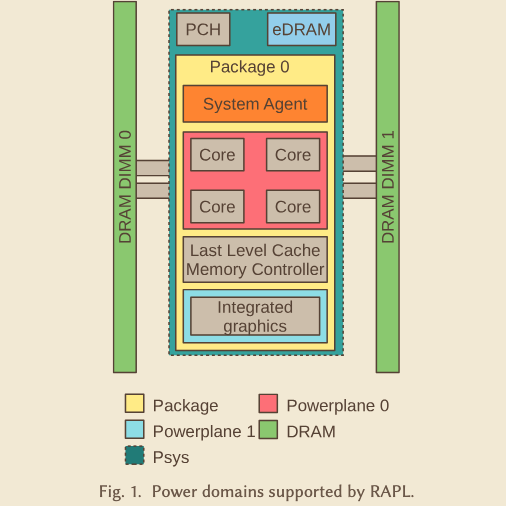
\includegraphics[width=0.6\linewidth]{figs/rapl-funcionamiento.png} % Imagen y anchura-altura de esta
    \caption{Dominio de estimación de métricas de consumo de RAPL junto con los grupos que lo componen y los componentes del sistema que abarca \cite{energy-rapl-mesurement}} %Titular ela imagen
    \label{fig:rapl-too-working} %Label para citar
 \end{figure}

\subsection{Estimar Consumo de la GPU}

La Graphics Processing Unit (GPU) es un componente diseñado para ejecutar operaciones de procesamiento de forma altamente paralela. A diferencia de las CPU, las GPU disponen de un elevado número de unidades de procesamiento que permiten ejecutar múltiples operaciones de forma simultánea, siendo especialmente adecuadas para cargas de trabajo con un elevado grado de paralelismo.

Existen dos tipos principales de GPU: las GPU discretas, que disponen de su propio chip de procesamiento, memoria y sistema de refrigeración y que normalmente se conectan a la placa base mediante PCI-Express; y las GPU integradas, que se encuentran integradas en el mismo chip que la CPU o en un SoC y que, generalmente, comparten la memoria principal del sistema.

La capacidad de procesamiento paralelo de las GPU ha favorecido su incorporación en diferentes ámbitos de computación, pasando de estar principalmente orientadas al procesamiento gráfico a utilizarse también en entornos de computación de altas prestaciones (\textit{High Performance Computing}, HPC) y centros de procesamiento de datos (CPD). Entre las cargas de trabajo que pueden beneficiarse de esta arquitectura se encuentran el procesamiento multimedia y, en particular, la codificación y decodificación de vídeo.

En este contexto, las GPU permiten trasladar determinadas operaciones desde la CPU hacia unidades de procesamiento especializadas, reduciendo potencialmente el tiempo de ejecución y el consumo energético asociado a determinadas cargas de trabajo. Esta capacidad resulta especialmente relevante en infraestructuras que procesan grandes cantidades de contenido multimedia, donde pequeñas diferencias en el consumo energético de cada proceso pueden representar un impacto significativo cuando las cargas se ejecutan de forma continua o simultánea.

Es por este motivo que la obtención de métricas de consumo energético precisas y con un nivel de granularidad adecuado es fundamental. Para llevar a cabo dicha toma de métricas, podría utilizarse un dispositivo físico; no obstante, al igual que sucede con la CPU, su uso en un entorno compuesto por numerosos nodos dificultaría en gran medida la instalación y gestión de los dispositivos. Es por ello que se opta por utilizar \textbf{nvidia-smi}, una herramienta de línea de comandos que se instala junto con los drivers y permite obtener métricas de la GPU. 

La herramienta \textit{nvidia-smi} se basa en la librería \textit{NVIDIA Management Library (NVML) \cite{nvml-api-officialdoc}}, que le permite tomar distintos tipos de métricas utilizando la API de la GPU. También sería posible utilizar NVML para estimar métricas de consumo energético, que \textit{nvidia-smi} ofrece mayores facilidades y ventajas \cite{nvidia-smi-documentation}. Cabe destacar que, dado que el software de NVIDIA es cerrado, no existe ningún análisis en profundidad que nos permita determinar el porqué de algunas de las métricas de resultado, más allá de la realización de experimentos y aplicar ingeniería inversa sobre los resultados. 

Basando los resultados obtenidos en el artículo \textit{Part-time Power Measurements: nvidia-smi’s lack of attention} \cite{gpu-measument-survery}, nvidia-smi puede obtener diversas métricas, entre las cuales se encuentran la potencia total gastada en un proceso y la energía (en un instante y a lo largo de un tiempo) de un proceso. No obstante, en el artículo se remarca que nvidia-smi tiene un pequeño tiempo de \textit{start-up} que ronda entre los \textbf{0 y los 100 milisegundos} y, por tanto, se debe iniciar la toma de métricas antes de lanzar el proceso del cual se desea monitorear el consumo energético. Con este ajuste, los investigadores destacan una reducción de la tasa de error que se encontraba en un $5\%$ a un $0\%$.



 